\selectlanguage{italian}%

\section{Soluzione}


\subsection{Schematici}

\begin{figure}[H]
	\centering
	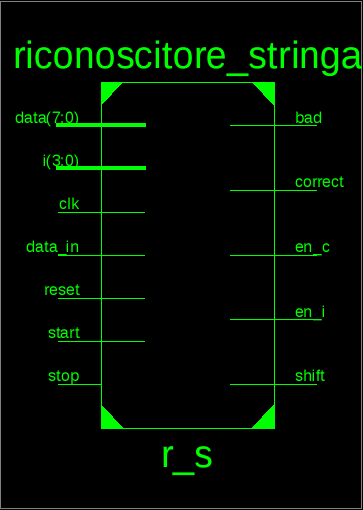
\includegraphics[scale=0.6]{esercizio07/images/riconoscitore_stringa.png}
	\caption{Riconoscitore di stringa}
\end{figure}

La macchina � composta semplicente da quattro stati:
\begin{itemize}
\item idle, in cui la macchina permane fintantoch� non viene avviata la
procedura di riconoscimento; 
\item carica\_stringa, in cui viene salvato in una scan chain il valore
della stringa da riconoscere;
\item shifting, in cui viene fatto shiftare il bit della stringa e far si
ponga in uscita alla scan\_chain; 
\item riconosci\_bit, si determina se il bit in uscita della scan\_chain
� uguale al bit della stringa da riconoscere ( quest' ultimo identificato
dal valore di un contatore che opportunamente identifica il valore
del bit da confrontare): se i due bit sono uguali, si procedere allo
shifting ed al riconoscimento fino a quando non vengono confrontati
tutti i bit ed un segnale indica che la stringa riconosciuta � proprio
quella voluta; altrimenti viene abilitato un segnale che indica il
fallimento della comparazione indicando la dissimilirit� della stringa
posta in ingresso da quella che si vuole riconoscere.
\end{itemize}

\subsection{Codice}


\subsubsection{Riconoscitore\_stringa}

\href{run:progetti/riconoscitore_stringa/riconoscitore_stringa.xise}{Riconoscitore Stringa ISE}

\smallskip{}

\lstinputlisting [language=VHDL,caption={Definizione della macchina a stati finiti},firstline=32] {progetti/riconoscitore_stringa/riconoscitore_stringa.vhd}

Notiamo che tutti i segnali di uscita, per le varie abilitazioni,
come lo shifting o l' abilitazione dei conteggi vengono fissati ad
un valore ben preciso prima del case all' interno del secondo process,
questo per far si che il sintetizzatore, non rilevi dei latch durante
la sua esecuzione, (ci� pu� essere dovuto al fatto che i segnali non
essendo fissati in dei registri il sintetizzatore vuole salvarli cos�
da poter effettuare una corretta sintesi del codice, questo vale anche
per le altre macchine a stati finiti sviluppate successivamente).

Di seguito vengono riportati i differenti risultati operativi nel
caso in cui si utilizzino diverse codifiche di rappresentazione degli
stati si una macchina a stati finiti.

\medskip{}

\noindent\begin{minipage}[t]{1\columnwidth}%
\begin{tabular}{|c|c|c|c|c|}
\hline 
Codifica & Numero di slice & Numero di flip flop & Numero di four lut & Frequenza massima\tabularnewline
\hline 
\hline 
One-hot & 19 & 16 & 37 & 184.805MHz\tabularnewline
\hline 
Speed1 & 19 & 16 & 37 & 184.805MHz\tabularnewline
\hline 
Compact & 15 & 14 & 29 & 191.031MHz\tabularnewline
\hline 
Sequential & 15 & 14 & 29 & 191.031MHz\tabularnewline
\hline 
Gray & 17 & 14 & 31 & 180.665MHz\tabularnewline
\hline 
Johnson & 17 & 14 & 31 & 180.665MHz\tabularnewline
\hline 
\end{tabular}%
\end{minipage}

\medskip{}

Dato il numero di stati molto ridotto, i risultati ottenuti utilizzando
le varie codifiche in alcuni casi sono risultati perfettamente gli
stessi, le codifiche che hanno dato gli stessi risultato sono state
messe una successivamente all' altra, difatti notiamo che One-hot
e Speed1 ottengono gli stessi risultati, facendo riferimento alla
manuale di XST di Xilinx la codifica Speed1 � orientata alla velocit�
ma i bit usati per identificare lo stato di solito sono in numero
maggiore al numero degli stati della macchina, quindi il sintetizzatore
alla fine si riconduce alla codica One-hot ed � quello che occupa
maggior area, dato che utilizza un singolo flip flop per codificare
ogni stato quindi la sua velocit� al crescere degli stati e indipendete,
anche se l' area occupata crescer� linearmente con il numero di stati;

compact � quella che richiede meno spazio cerca di utilizzare il minore
numero di bit possibili per codificare gli stati, in questo caso risulta
la pi� efficiente, perch� oltre ad essere minore lo spazio occupato
essendo il numero di stati davvero esiguo il tutto riesce ad essere
mappato in slice presenti nella stessa CLB, rendendo la frequenza
massima operativa maggiore;

Sequential utilizzato un approccio radix-two sugli stati presenti
su path molto lunghi, ma in questo caso ci si riconduce ad una soluzione
compact essendo gli stati solo due; 

Gray permetteno di far variare un solo bit alla volta occupa lo stesso
spazio della compact, ma la logica combinatoriale per far variare
tra gli stati e pi� complessa ed implica anche una minore frequenza
operativa, per rendere sicuro il cambio di stato;

Johnson comunque permette la variazione di un solo bit alla volta,
ma in questo caso coincide con la codifica di gray, anche se di solito
i bit per la rappresentazione sono maggiori.\selectlanguage{italian}%

